\documentclass[a4paper,12pt]{article}
\usepackage[left=2cm,right=1cm,top=1cm,bottom=1.5cm]{geometry}
\usepackage[utf8]{inputenc}
\usepackage[english,russian]{babel}
\usepackage{graphicx}
\usepackage{amsmath}
\usepackage{amssymb}
\usepackage{cite}
\usepackage{indentfirst}
\usepackage{multicol}
\usepackage{cmap}
\usepackage{hyperref}
\usepackage{esint}
\usepackage{listings}
%\usepackage{minted}
\usepackage{xcolor}
\usepackage[T1]{fontenc}
\usepackage{drftcite}
\usepackage{pdfpages}
%\usepackage{inconsolata}
%\renewcommand*\familydefault{\ttdefault} %% Only if the base font of the document is to be typewriter style
%\usepackage[T1]{fontenc}
\hypersetup{
	colorlinks=true,
	linkcolor=black,
	filecolor=black,  
	urlcolor=blue,
	pdftitle={Overleaf Example},
	pdfpagemode=FullScreen,
}

\sloppy

\geometry{top=2cm}
\geometry{bottom=2cm}
\geometry{left=2.5cm}
\geometry{right=2.5cm}

\renewcommand{\baselinestretch}{1.5}

	\newcommand{\ds}{\displaystyle}
	\renewcommand{\phi}{\varphi}
	\newcommand{\sgn}{\, \text{sgn} \,}
	\renewcommand{\a}{\alpha}
	\renewcommand{\b}{\beta}
	\renewcommand{\l}{\lambda}
	\renewcommand{\d}{\partial}
	\newcommand{\e}{\varepsilon}
	\renewcommand{\^}[2]{#1^{\, #2} \kern -1pt}
	\newcommand{\veco}{\kern -1pt \vec{\kern 1pt 0}}
	\newcommand{\1}{\kern 1pt}
	\newcommand{\0}{\kern -1pt}
	%\renewcommand{\Phi}{\varPhi}
	
\newcommand{\vs}{\vspace{0.2cm}}
	
	
\begin{document}
	
	\begin{titlepage}
		\begin{center}
			\small{Национальный исследовательский ядерный университет «МИФИ»}\\*
		\end{center}
		\vspace{7cm}
		
		\begin{center}
			\Large{\textbf{Задание по курсу}\\
				\textbf{«Теория управления»}}
		\end{center}
		\vspace{2cm}
		
		\begin{flushright}
			Выполнил\\
			студент группы Б21-215\\
			Бородин Михаил Сергеевич\\
			\vspace{0.5cm}
			Вариант №5
		\end{flushright}
		\vspace{8cm}
		
		\begin{center}
			\textbf{2023}
		\end{center}
	\end{titlepage}


	\newpage 
	\setcounter{page}{2}
	
	
	Исходная структурная схема линейной динамической системы:
	
	\begin{center}
		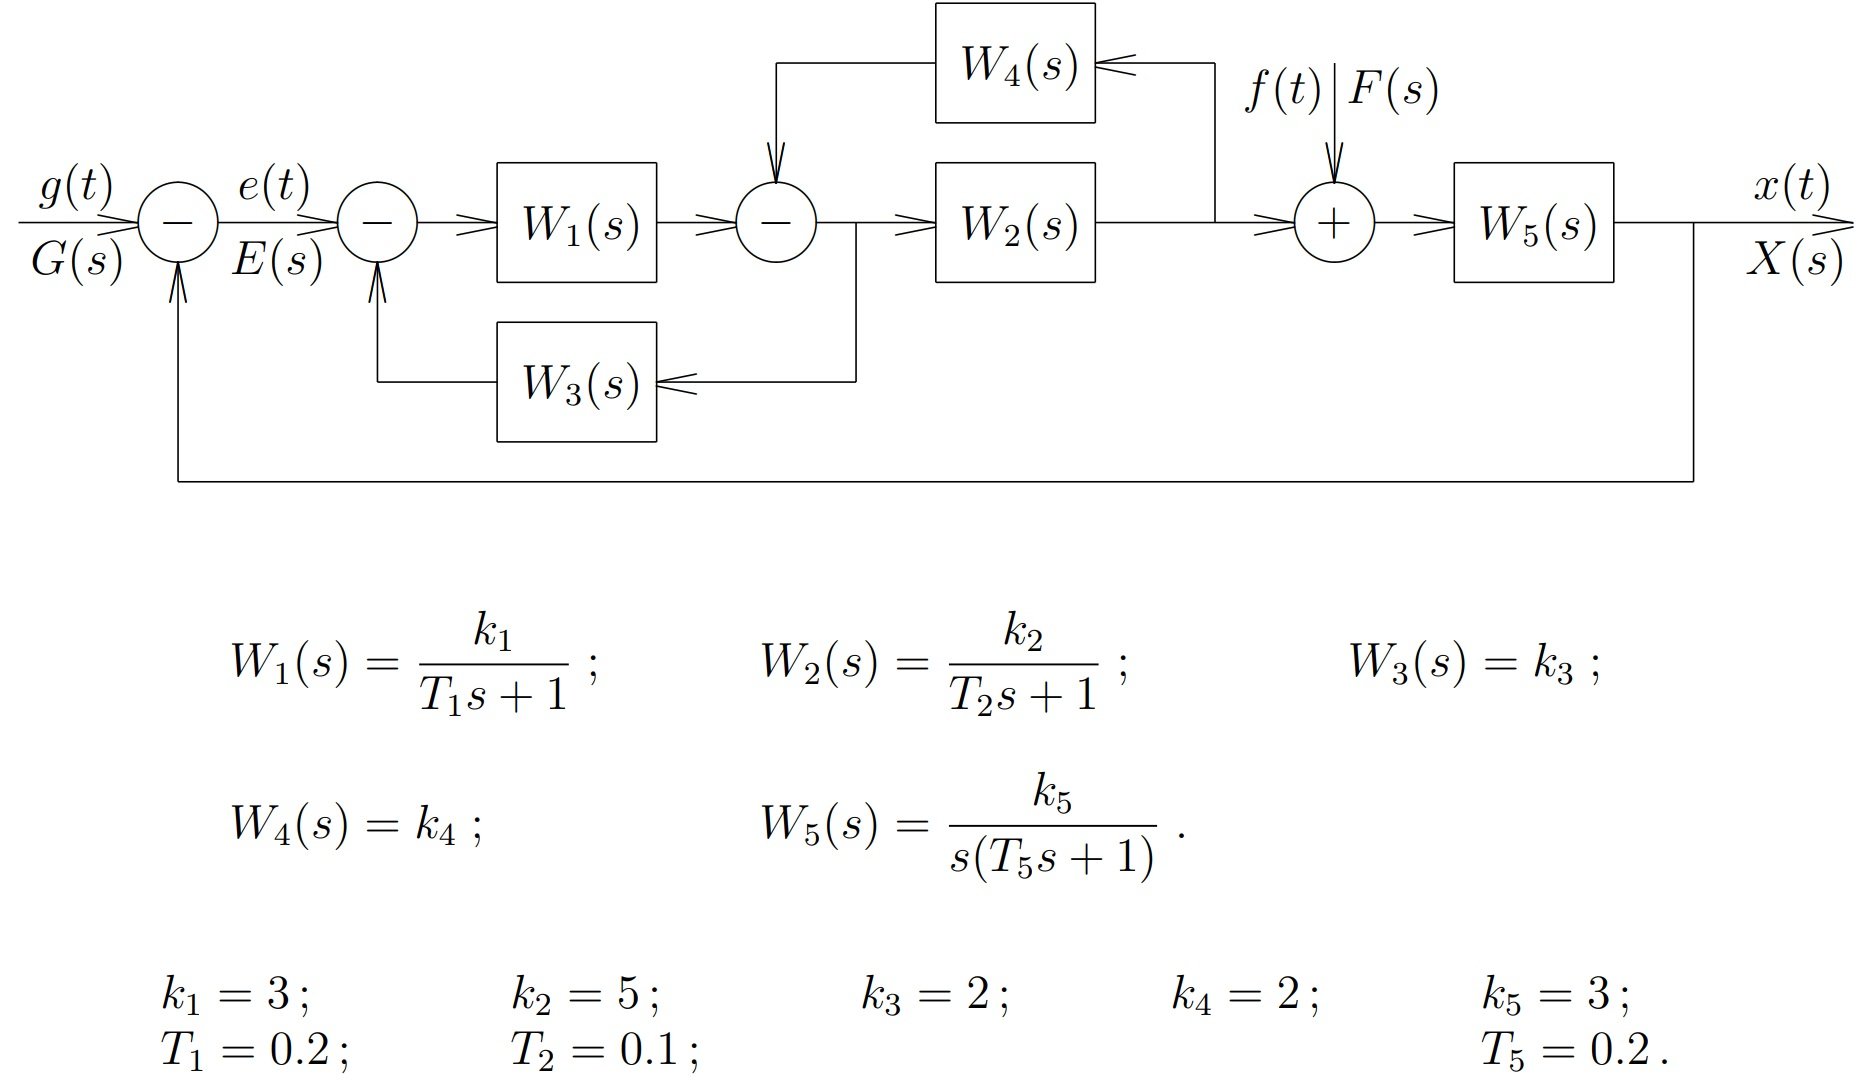
\includegraphics[scale=0.6,page=1]{исходная_схема}
	\end{center}
	%$\\$
	
	\newpage
	
	\textbf{Задание 1.} Составить уравнения динамики разомкнутой и замкнутой систем в пространстве состояний (определить матрицу $A$, векторы $\overline{b}$, $\overline{c}^T$, коэффициент $d$).
	$\\$
	
	Для разомкнутой схемы:
	
	\begin{center}
		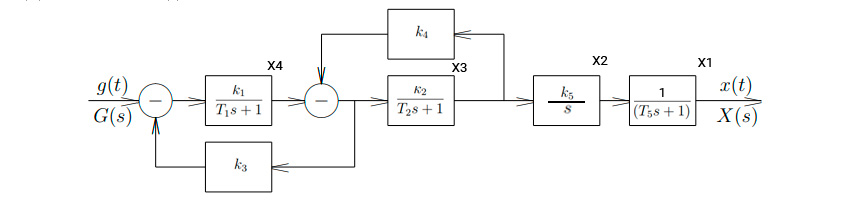
\includegraphics[scale=0.6,page=1]{1_зад/подставлено в разомкнутую}
	\end{center}
	
	$\ds \mathrm{x}_1 = x$
	
	$\ds T_5 \frac{d \mathrm{x}_1}{dt} + \mathrm{x}_1 = \mathrm{x}_2$
	\vs
	
	$\ds \frac{d \mathrm{x}_2}{dt} = k_5 \mathrm{x}_3 $
	\vs
	
	$\ds T_2  \frac{d \mathrm{x}_3}{dt} + \mathrm{x}_3 = k_2 \bigg(\mathrm{x}_4 - k_4 \mathrm{x}_3  \bigg)$
	\vs

	$\ds T_1  \frac{d \mathrm{x}_4}{dt} + \mathrm{x}_4 = k_1 \bigg(g - k_3 (\mathrm{x}_4 - k_4 \mathrm{x}_3) \bigg)$
	
	$\\$
	
%	Отсюда уравнение динамики разомкнутой системы:
	
	$\begin{cases}
		\ds \frac{d \mathrm{x}_1}{dt} = - \frac{1}{T_5} \mathrm{x}_1 + \frac{1}{T_5} \mathrm{x}_2 \\
		\ds \frac{d \mathrm{x}_2}{dt} = k_5 \mathrm{x}_3 \\
		\ds \frac{d \mathrm{x}_3}{dt} = - \frac{1 + k_2 k_4}{T_2} \mathrm{x}_3 + \frac{k_2}{T_2} \mathrm{x}_4 \\
		\ds \frac{d \mathrm{x}_4}{dt} = \frac{k_1 k_3 k_4}{T_1} \mathrm{x}_3 - \frac{1 + k_1 k_3}{T_1} \mathrm{x}_4 + \frac{k_1}{T_1} g \\
	\end{cases}$
	\vs
	
	$\ds \mathrm{x}_1 = x$
	$\\$
	
	$\ds A = \begin{pmatrix}
		- \frac{1}{T_5} & \frac{1}{T_5} & 0 & 0 \\
		0 & 0 & k_5 & 0 \\
		0 & 0 & - \frac{1 + k_2 k_4}{T_2} & \frac{k_2}{T_2} \\
		0 & 0 & \frac{k_1 k_3 k_4}{T_1} & - \frac{1 + k_1 k_3}{T_1}
	\end{pmatrix}$\hspace{1.0cm}
	$\ds \overline{b} = \begin{pmatrix}
		0 \\
		0 \\
		0 \\
		\frac{k_1}{T_1}
	\end{pmatrix}$\hspace{1.0cm}
	$\ds \overline{c}^T = \begin{pmatrix} 1 & 0 & 0 & 0 \end{pmatrix}$\hspace{1.0cm}
	$\ds d = 0$
	
	$\\$
	
	$\ds A = \begin{pmatrix}
		- 5 & 5 & 0 & 0 \\
		0 & 0 & 3 & 0 \\
		0 & 0 & - 110 & 50 \\
		0 & 0 & 60 & - 35
	\end{pmatrix}$\hspace{1.0cm}
	$\ds \overline{b} = \begin{pmatrix}
		0 \\
		0 \\
		0 \\
		15
	\end{pmatrix}$\hspace{1.0cm}
	$\ds \overline{c}^T = \begin{pmatrix} 1 & 0 & 0 & 0 \end{pmatrix}$\hspace{1.0cm}
	$\ds d = 0$
	%$\\$
	\newpage
	
	
	Для замкнутой схемы:
	
	\begin{center}
		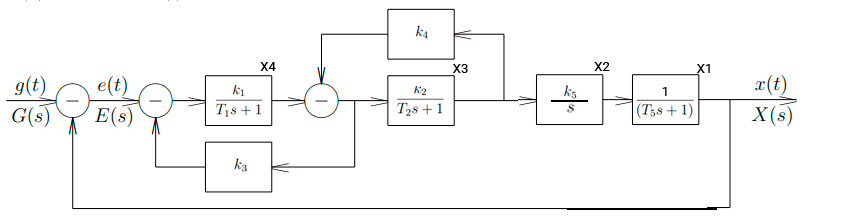
\includegraphics[scale=0.6,page=1]{1_зад/подставлено в исходную без внешнего воздейтсвия}
	\end{center}

	$\ds \mathrm{x}_1 = x$

	$\ds T_5 \frac{d \mathrm{x}_1}{dt} + \mathrm{x}_1 = \mathrm{x}_2$
	\vs

	$\ds \frac{d \mathrm{x}_2}{dt} = k_5 \mathrm{x}_3 $
	\vs

	$\ds T_2  \frac{d \mathrm{x}_3}{dt} + \mathrm{x}_3 = k_2 \bigg(\mathrm{x}_4 - k_4 \mathrm{x}_3  \bigg)$
	\vs

	$\ds T_1  \frac{d \mathrm{x}_4}{dt} + \mathrm{x}_4 = k_1 \bigg(g - \mathrm{x}_1 - k_3 (\mathrm{x}_4 - k_4 \mathrm{x}_3) \bigg)$

	$\\$
	$\begin{cases}
		 \ds \frac{d \mathrm{x}_1}{dt} = - \frac{1}{T_5} \mathrm{x}_1 + \frac{1}{T_5} \mathrm{x}_2 \\
		 \ds \frac{d \mathrm{x}_2}{dt} = k_5 \mathrm{x}_3 \\
		 \ds \frac{d \mathrm{x}_3}{dt} = - \frac{1 + k_2 k_4}{T_2} \mathrm{x}_3 + \frac{k_2}{T_2} \mathrm{x}_4 \\
		 \ds \frac{d \mathrm{x}_3}{dt} = - \frac{k_1}{T_1} \mathrm{x}_1 +  \frac{k_1 k_3 k_4}{T_1} \mathrm{x}_3 - \frac{1 + k_1 k_3}{T_1} \mathrm{x}_4 + \frac{k_1}{T_1} g \\
	\end{cases}$
	\vs

	$\ds \mathrm{x}_1 = x$
	$\\$

	$\ds A = \begin{pmatrix}
				 - \frac{1}{T_5} & \frac{1}{T_5} & 0 & 0 \\
				 0 & 0 & k_5 & 0 \\
				 0 & 0 & - \frac{1 + k_2 k_4}{T_2} & \frac{k_2}{T_2} \\
				 - \frac{k_1}{T_1} & 0 & \frac{k_1 k_3 k_4}{T_1} \mathrm{x}_3 & - \frac{1 + k_1 k_3}{T_1}
	\end{pmatrix}$\hspace{1.0cm}
	$\ds \overline{b} = \begin{pmatrix}
							0 \\
							0 \\
							0 \\
							\frac{k_1}{T_1}
	\end{pmatrix}$\hspace{1.0cm}
	$\ds \overline{c}^T = \begin{pmatrix} 1 & 0 & 0 & 0 \end{pmatrix}$\hspace{1.0cm}
	$\ds d = 0$

	$\\$

	$\ds A = \begin{pmatrix}
				 - 5 & 5 & 0 & 0 \\
				 0 & 0 & 3 & 0 \\
				 0 & 0 & - 110 & 50 \\
				 -15 & 0 & 60 & - 35
	\end{pmatrix}$\hspace{1.0cm}
	$\ds \overline{b} = \begin{pmatrix}
							0 \\
							0 \\
							0 \\
							15
	\end{pmatrix}$\hspace{1.0cm}
	$\ds \overline{c}^T = \begin{pmatrix} 1 & 0 & 0 & 0 \end{pmatrix}$\hspace{1.0cm}
	$\ds d = 0$
	
	
	\newpage
	
	\textbf{Задание 2.} Определить передаточную функцию разомкнутой системы $W(s)$, приведя ее к типовым звеньям. Построить ЛАФЧХ разомкнутой системы на ЛАХ-бумаге. Определить передаточную функцию замкнутой системы $\Phi(s)$.
	$\\$
	
	Разомкнутая система:
	
	\begin{center}
		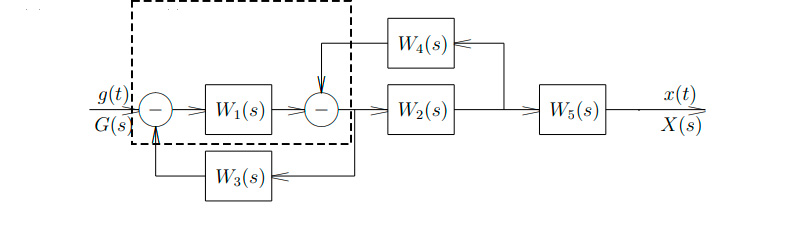
\includegraphics[scale=0.5,page=1]{Преобразования/1}
	\end{center}
	%$\\$

	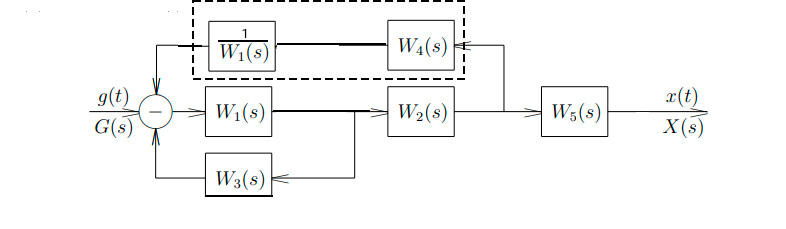
\includegraphics[scale=0.5,page=1]{Преобразования/2}
	$\\$

	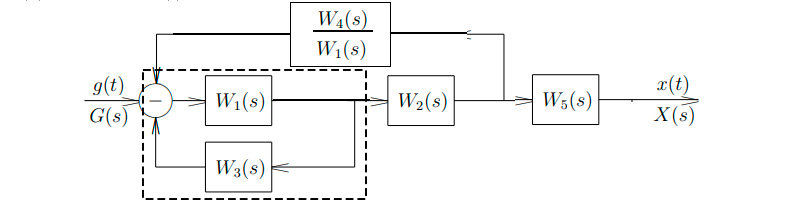
\includegraphics[scale=0.5,page=1]{Преобразования/3}
	$\\$
	
	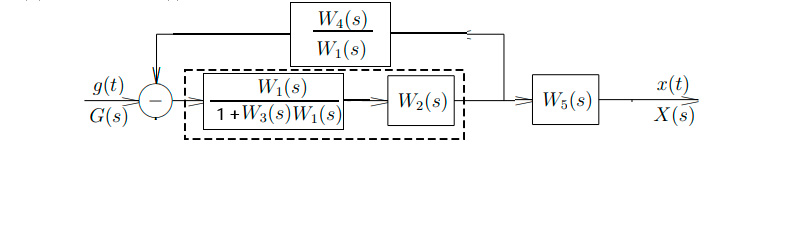
\includegraphics[scale=0.5,page=1]{Преобразования/4}
	$\\$
	
	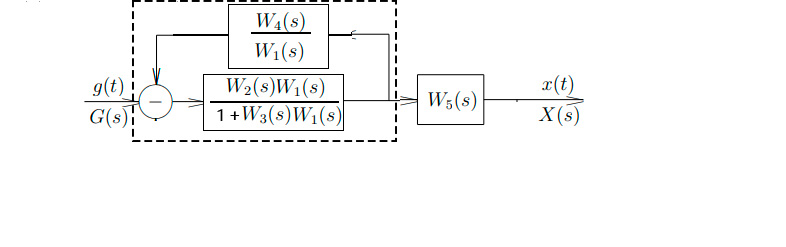
\includegraphics[scale=0.5,page=1]{Преобразования/5}
	$\\$
	
	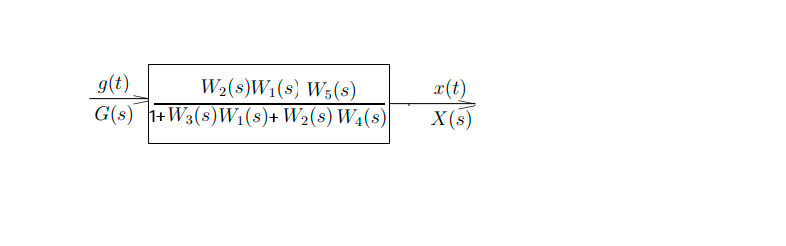
\includegraphics[scale=0.5,page=1]{Преобразования/6}
	$\\$

	$\ds W(s) = \frac{W_1(s) W_2(s) W_5(s)}{1 + W_1(s) W_3(s) + W_2(s) W_4(s)}
	= \frac{\frac{k_1}{T_1 s + 1} \cdot \frac{k_2}{T_2 s + 1} \cdot \frac{k_5}{s (T_5 s + 1)} }{1 + \frac{k_1}{T_1 s + 1} \cdot k_3 + \frac{k_2}{T_2 s + 1} \cdot k_4} = $
	\vs
	
	$\ds = \frac{45}{17} \cdot \frac{1}{s} \cdot \frac{1}{0.2 s + 1} \cdot \frac{1}{\frac{2}{1700} s^2 + \frac{29}{170} s + 1}$
	$\\$

	ЛАФЧХ разомкнутой системы (вместе с асимптотическими графиками):
	
	\begin{center}
%		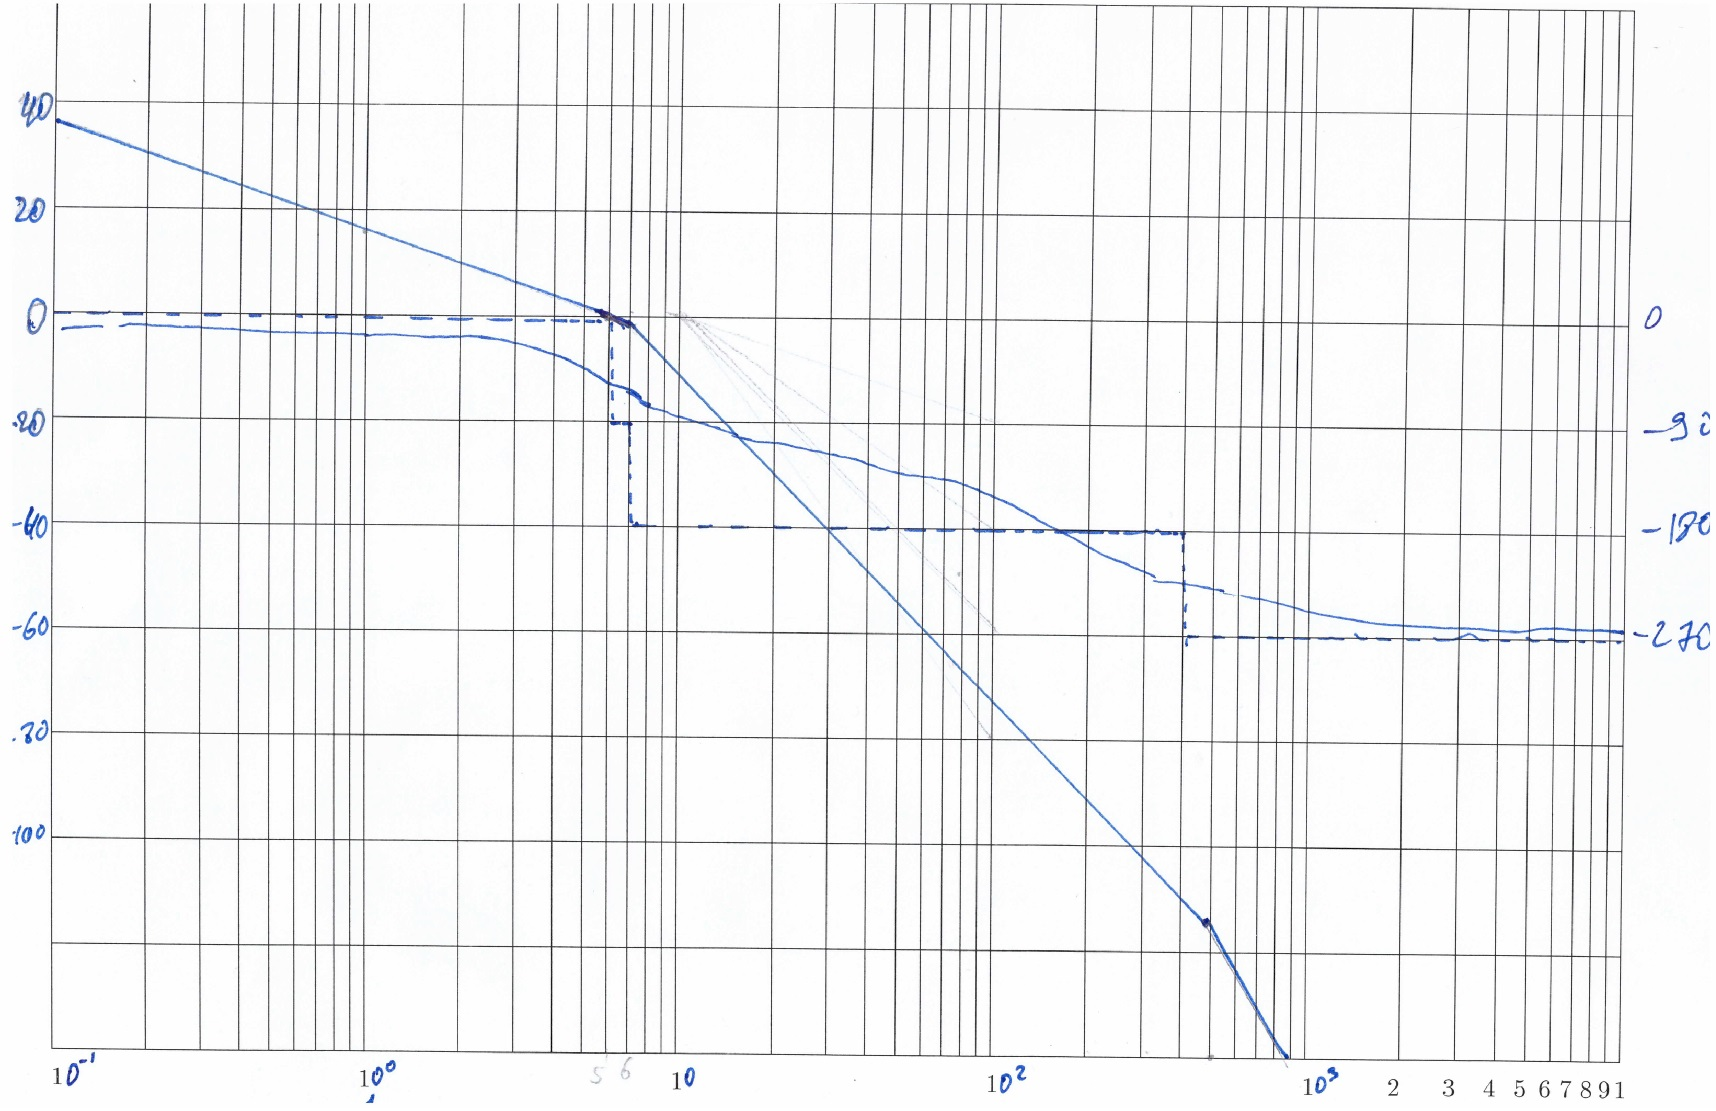
\includegraphics[scale=0.7,page=1]{лачх_лфчх}
		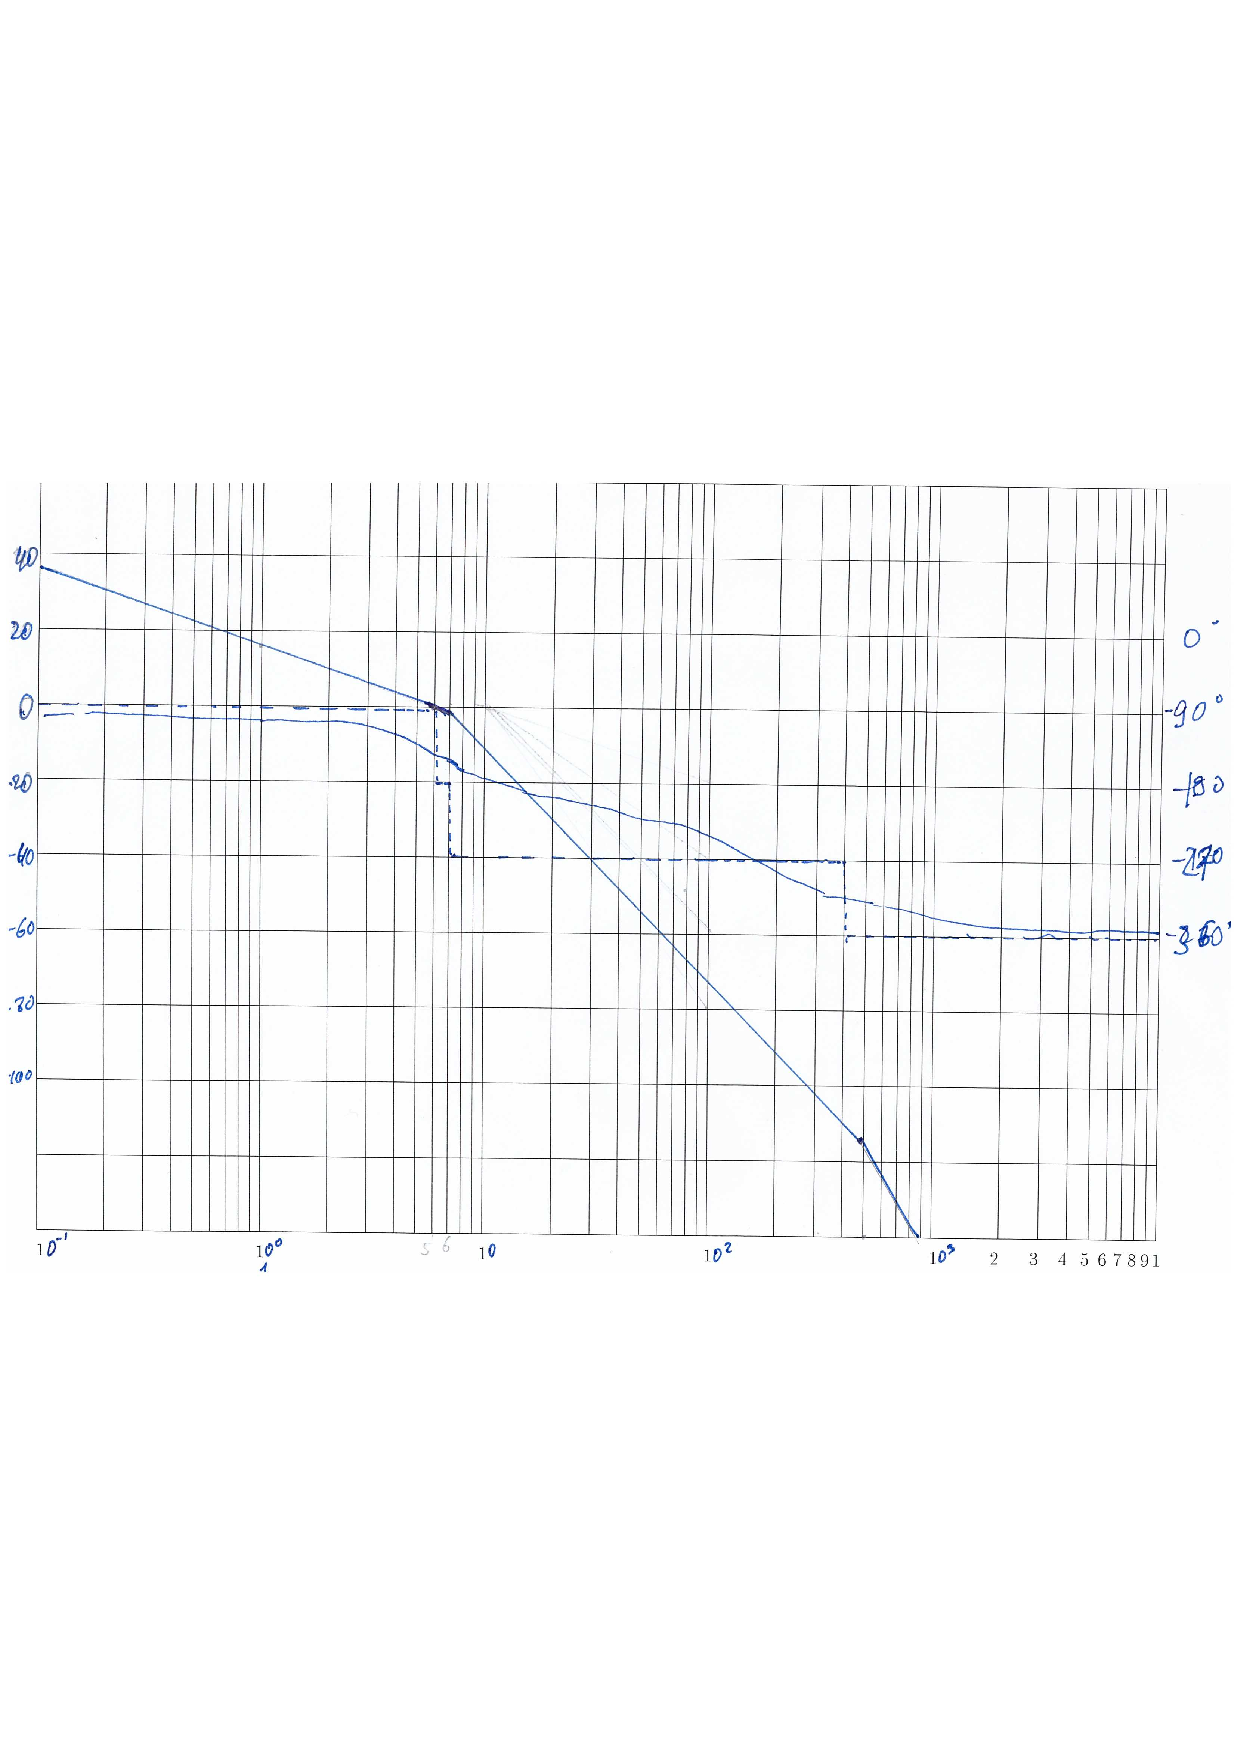
\includepdf{лачх_от_руки}
	\end{center}
	
	Замкнутая система:
	
	\begin{center}
		
\includegraphics[scale=1,page=1]{Преобразования/Схема_преобр_7}
	\end{center}
	
	$\ds \Phi(s) = \frac{W(s)}{1 + W(s)} = \frac{\frac{45}{17} \cdot \frac{1}{s} \cdot \frac{1}{0.2 s + 1} \cdot \frac{1}{\frac{2}{1700} s^2 + \frac{29}{170} s + 1}}{1 + \frac{45}{17} \cdot \frac{1}{s} \cdot \frac{1}{0.2 s + 1} \cdot \frac{1}{\frac{2}{1700} s^2 + \frac{29}{170} s + 1}} = $
	\vs
	
	$\ds = \frac{1}{\frac{1}{11250} s^4 + \frac{1}{75} s^3 + \frac{7}{50} s^2 + \frac{17}{45} s + 1}$
	
	\newpage
	
	\textbf{Задание 3.} Построить на компьютере АФЧХ (годограф) и ЛАФЧХ разомкнутой и замкнутой систем.
	$\\$
	
	ЛАФЧХ разомкнутой системы:
	\begin{center}
		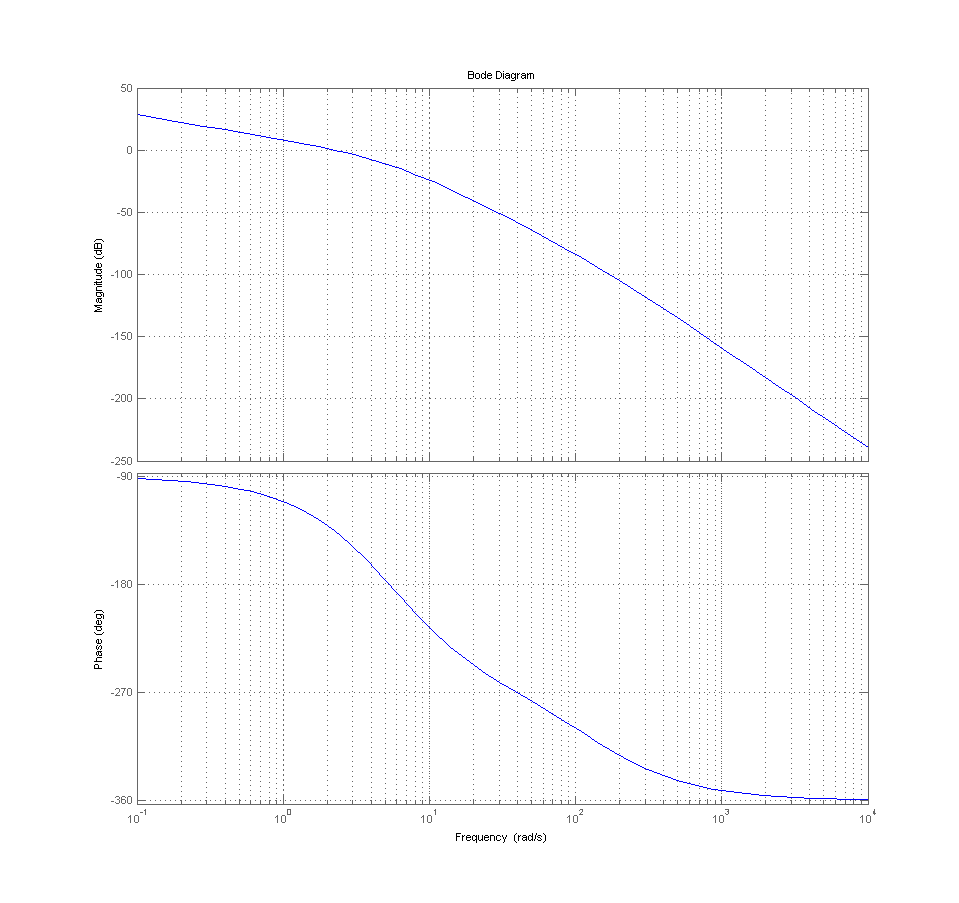
\includegraphics[scale=0.7,page=1]{3_зад/bode_разомкнутой}
	\end{center}
	\newpage
	
	ЛАФЧХ замкнутой системы:

	\begin{center}
		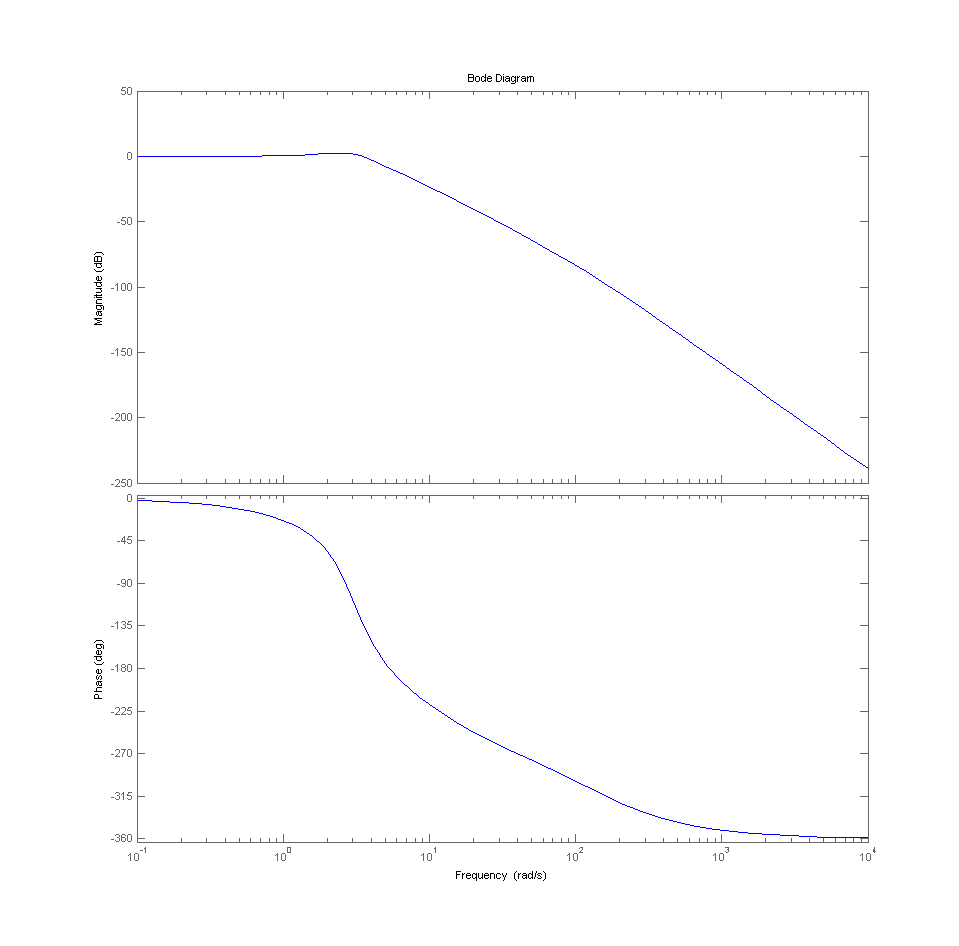
\includegraphics[scale=0.7,page=1]{3_зад/bode_замкнутой}
	\end{center}
	
	\newpage
	
	АФЧХ (годограф) разомкнутой системы:

	\begin{center}
		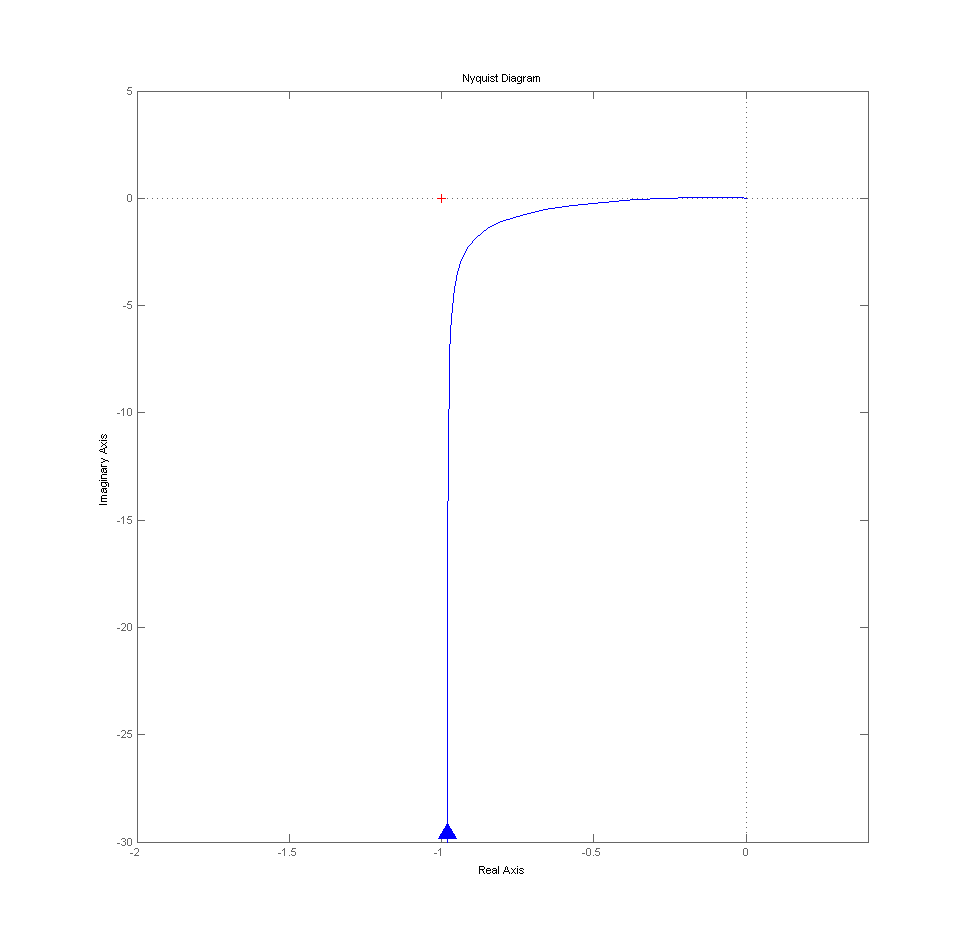
\includegraphics[scale=0.7,page=1]{3_зад/nyquist_разомкнутой(2)}
	\end{center}

	\newpage
	АФЧХ (годограф) замкнутой системы:

	\begin{center}
		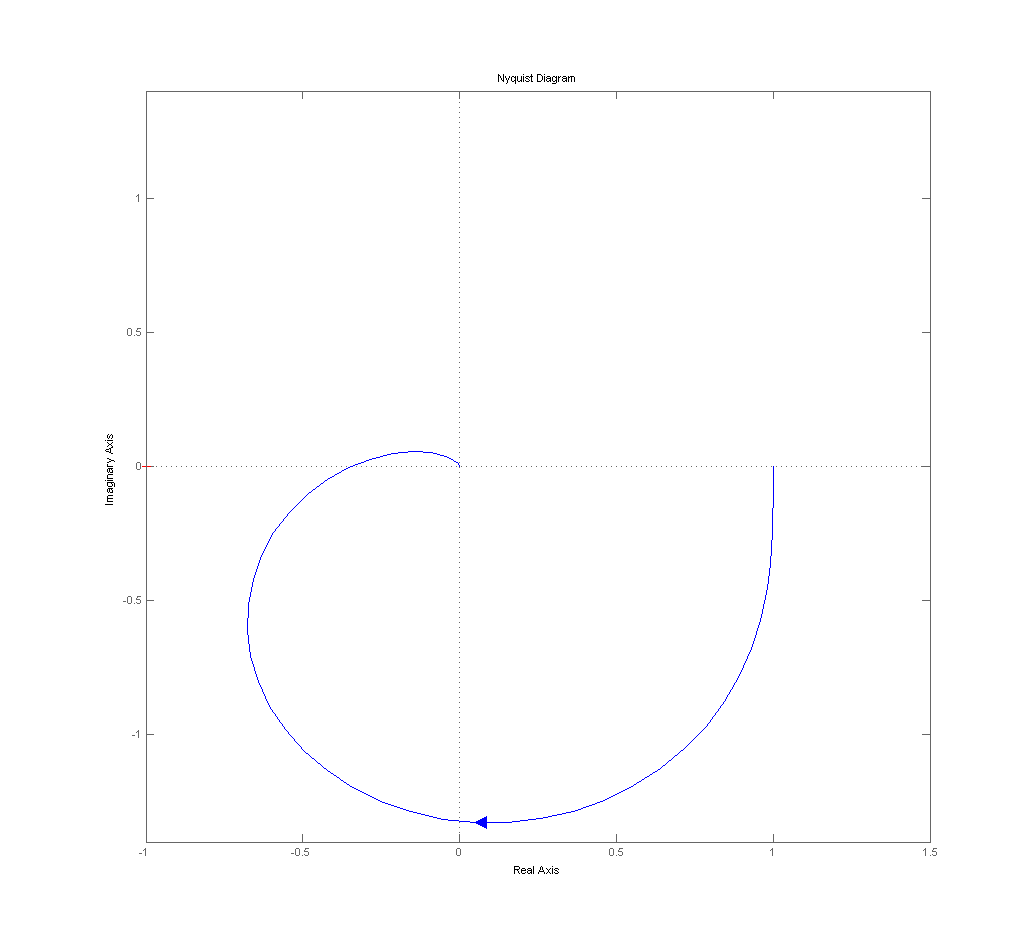
\includegraphics[scale=0.4,page=1]{3_зад/nyquist_замкнутой}
	\end{center}
	
	
	\newpage
	
	\textbf{Задание 4.} Исследовать устойчивость системы с использованием ЛАФЧХ и частотного критерия. Определить предельный коэффициент усиления системы, при котором система находится на грани устойчивости.
	$\\$
	
	По критерию Найквиста: для устойчивости замкнутой ЛДС необходимо и достаточно, чтобы её годограф в разомкнутом состоянии охватывал критическую точку $(-1; 0 j)$ против часовой стрелки $K/2$ раз при возрастании частоты $0 \leqslant \omega < +\infty$, где $K$ -- число полюсов передаточной функции разомкнутой системы в правой полуплоскости.
	$\\$
	
	Передаточная функция разомкнутой системы:
	\vs

	$\ds = \frac{45}{17} \cdot \frac{1}{s} \cdot \frac{1}{0.2 s + 1} \cdot \frac{1}{\frac{2}{1700} s^2 + \frac{29}{170} s + 1}$
	\vs
	
	Полюсы $W(s)$: \; $\ds \l_1 = 0$, \, $\ds \l_2 = - 5$, \, $\ds \l_3 \approx - 5.98 $  \, $\ds \l_4 \approx - 284.01$.
	Ни один из полюсов не расположен в правой полуплоскости, так что $K = 0$.

	\begin{center}
		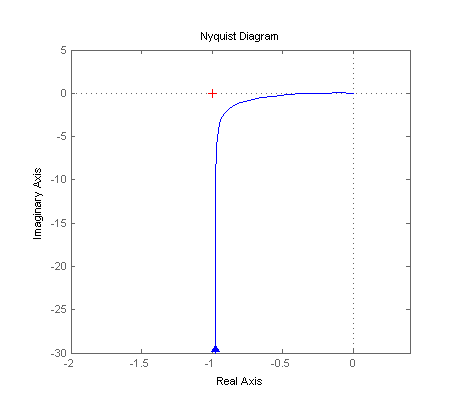
\includegraphics[scale=0.7,page=1]{4_зад/nyquist_разомкнутой(2)_маленький}
	\end{center}
	
	Из построенного рисунка видно, что годограф не охватывает точку $(-1,0 j)$ (т. е. охватывает её 0 раз). Поэтому выполняется равенство:
	
	$\ds 0 = \frac{0}{2}$ -- то есть система устойчива.
	
	
	Сделаем коэффициент усиления звеньев $\ds k = \frac{45}{17}$ варьируемой переменной:
	\vs
	
	$\ds W(s) = k \;  \cdot \frac{1}{s} \cdot \frac{1}{0.2 s + 1} \cdot \frac{1}{\frac{2}{1700} s^2 + \frac{29}{170} s + 1}$
	$\\$
	
	Тогда ЛАЧХ данной передаточной функции будет совершать вертикальный параллельный перенос при изменении значения k.
	\begin{center}
		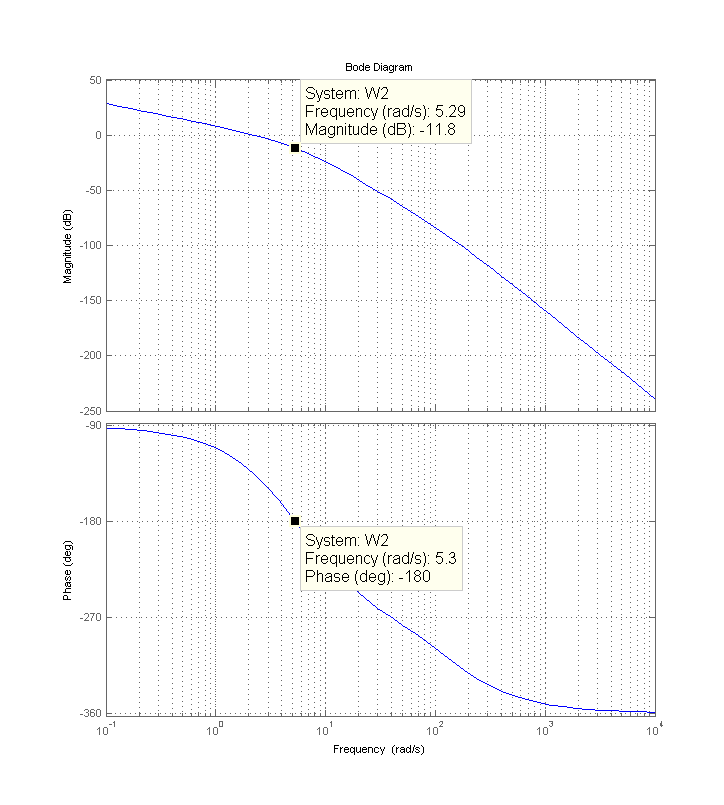
\includegraphics[scale=0.6,page=1]{4_зад/nyquist_разомкнутой_исседование1}
	\end{center}
	Из рисунка видно, что запас устойчивости по амплитуде $h_m \approx 11.8$ -- на такую величину можно параллельно переносить ЛАЧХ вверх, прежде чем её точка пересечения с нулём окажется правее, чем точка пересечения ФЧХ со значением $-180$, в случае чего система уже окажется неустойчивой.
	
	Тогда:
	
	$\ds 20 \lg k_{\text{кр}} = 20 \lg \frac{45}{17} + h_m$
	
	$\ds k_{\text{кр}} = \frac{45}{17} \cdot 10^{h_m/20} \approx 10$ -- при таком $k$ система находится на грани устойчивости.
	
	\hspace{-2.0cm}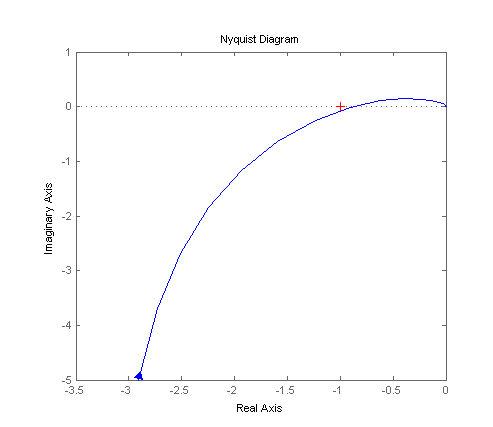
\includegraphics[scale=0.75,page=1]{4_зад/nyquist_разомкнутой_исседование_k9}
	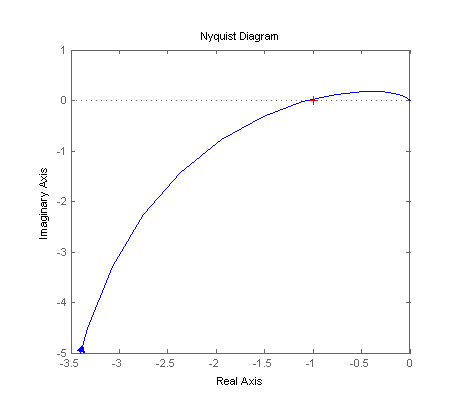
\includegraphics[scale=0.8,page=1]{4_зад/nyquist_разомкнутой_исседование_k11}
	
	Выше приведены АФЧХ для случаев $k = 9$ и $k = 11$ соответственно.
	Видно, что в первом случае годограф не охватывает точку $(-1,0 j)$ (т. е. охватывает её 0 раз), поэтому выполняется равенство $\ds 0 = \frac{0}{2}$, и система оказывается устойчивой.
	А во втором случае годограф охватывает точку $(-1,0 j)$ 1 раз по часовой стрелке (т. е. охватывает $-1$ раз против часовой стрелки), поэтому выражение $\ds -1 = \frac{0}{2}$ не является равенством, и система оказывается неустойчивой.
	
	
	\newpage
	
	\textbf{Задание 5.} Построить на компьютере переходные процессы в замкнутой системе при действии единичного ступенчатого, линейного нарастающего и гармонического воздействий. Определить астатизм, коэффициенты добротности системы и предельные значения установившихся ошибок при $g(t) = 1 [t]$, $g(t) = at$. Определить коэффициенты ошибок $C_0$, $C_1$, $C_2$.
	$\\$
	
	Для построения переходных процессов при заданных воздействиях использовалась команда \texttt{lsim(sys,g,t)} в среде MATLAB.
	$\\$
	
	Переходный процесс при действии единичного ступенчатого воздействия:

	\begin{center}
		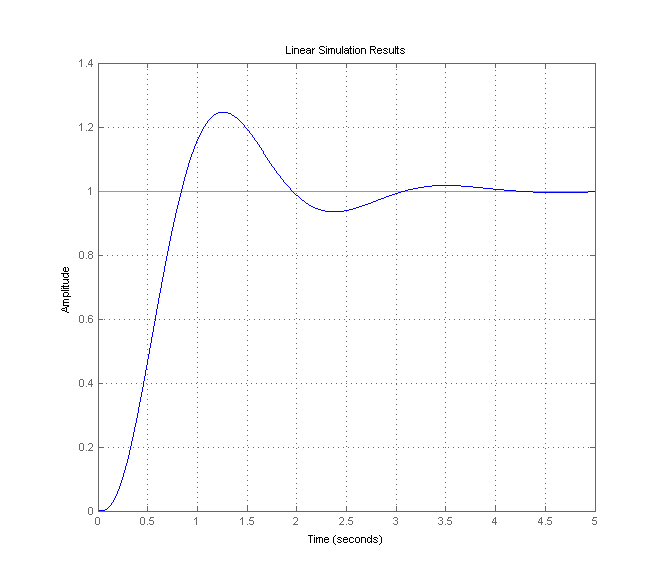
\includegraphics[scale=0.7,page=1]{5_зад_переходные_процессы/переходный_процесс_скачок}
	\end{center}

			\vs
	
	Переходный процесс при действии линейного нарастающего воздействия:

	\begin{center}
		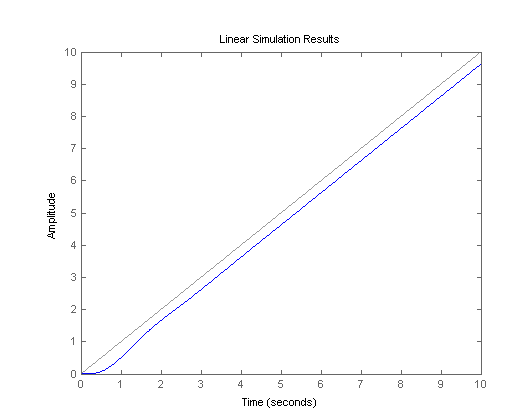
\includegraphics[scale=0.7,page=1]{5_зад_переходные_процессы/переходный_процесс_линейный}
	\end{center}

	Переходный процесс при действии гармонического воздействия:

	\begin{center}
		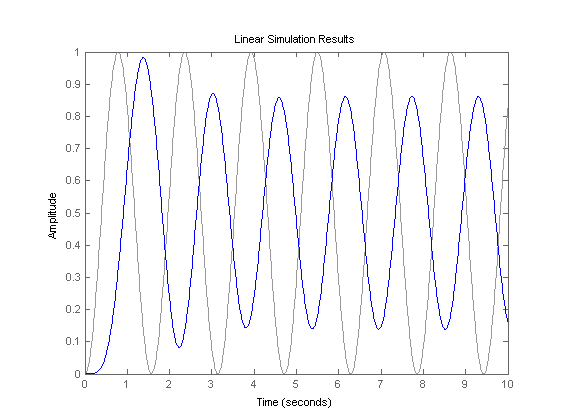
\includegraphics[scale=0.7,page=1]{5_зад_переходные_процессы/переходный_процесс_синус}
	\end{center}

	$\\$
	
	Передаточная функция разомкнутой системы:
	\vs
	
	$\ds W(s) = \frac{45}{17} \cdot \frac{1}{s} \cdot \frac{1}{0.2 s + 1} \cdot \frac{1}{\frac{2}{1700} s^2 + \frac{29}{170} s + 1}$
	\vs
	
	В системе имеется одно интегрирующее звено, значит, система имеет \textbf{астатизм первого порядка}.
	
	$\nu = 1$
	$\\$
	
	%Коэффициент добротности по положению $\ds k_p = 1 + k = \frac{13}{3}$.
	
	Коэффициент добротности по скорости $\ds k_v = k = \frac{45}{17}$.
	%
	%Коэффициент добротности по ускорению $\ds k_a = k = \frac{10}{3}$.
	$\\$
	
	Передаточная функция замкнутой системы относительно ошибки $\e(t)$:
	\vs
	
	$\ds \Phi_\e(s) = \frac{1}{1 + W(s)} = \frac{1}{\frac{1}{11250} s^4 + \frac{1}{75} s^3 + \frac{7}{50} s^2 + \frac{17}{45} s + 1} $
	\vs
	
	$\\$
	
	Коэффициенты ошибок:
	
	$\ds C_0 = \Phi_\e(0) = 1 $
	
	$\ds C_1 = \frac{d \Phi_\e}{ds} \bigg|_{s=0} \approx -0.378 $
	
	$\ds C_2 = \frac{d^2 \Phi_\e}{ds^2} \bigg|_{s=0}  \approx 0.0054 $
	$\\$
	
	Предельные значения установившихся ошибок:
	\vs
	
	$\ds \e(t) = C_0 g(t) + \frac{C_1}{1!} \frac{dg(t)}{dt} + \frac{C_2}{2!} \frac{d^2 g(t)}{dt^2} + \dots$
	\vs
	
	$\ds g(t) = 1 [t]$: \;\; $\ds \e(t) = C_0 = 1$
	\vs
	
	$\ds g(t) = at$: \;\; $\ds \e(t) = C_0 a t + C_1 a = -0.378 a$
	
	\newpage

	\textbf{Задание 6.} Синтезировать последовательное корректирующее устройство по заданным показателям качества. Построить на компьютере переходный процесс в скорректированной системе при действии единичного ступенчатого воздействия.

	Показатели качества: \hspace{1.0cm} $t_{\text{р}} = 0.03$ с \hspace{1.0cm} $\sigma_{\max} = 15 \%$
	$\\$

	Желаемая передаточная функция подбиралась в виде:

	$\ds W_{\text{ж}}(s) = k \; \frac{1}{s} \; \frac{1}{T s + 1}$
	\vs

	В результате подбора получилось добиться передаточной функции, которая полностью удовлетворяет показателям качества:

	$\ds W_{\text{ж}}(s) = 185 \; \frac{1}{s} \; \frac{1}{0.005 s + 1}$
	\vs

	Переходный процесс при действии единичного ступенчатого воздействия:

	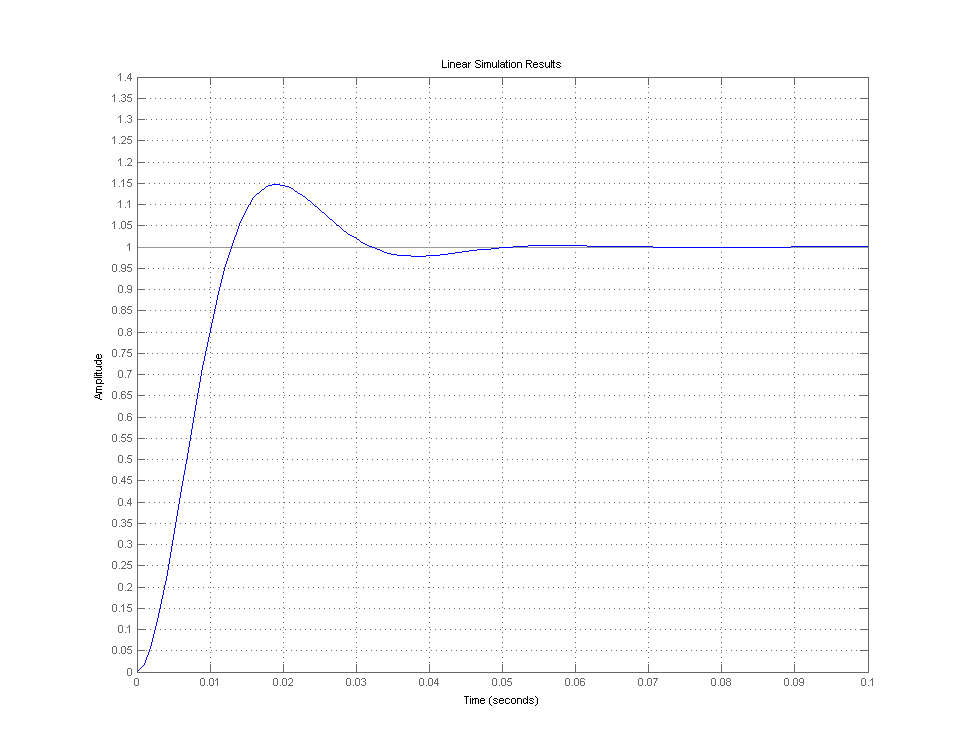
\includegraphics[scale=0.7,page=1]{6_зад/скачок_подобранная}

	В данном случае время регулирования $t_{\text{р}} = 0.027$ с, перерегулирование $\sigma_{\max} = 15 \%$, частота среза $\ds \omega_{\text{с}} = 185$.
	$\\$

	$\ds W_{\text{ж}}(s) = W_{\text{н}}(s) \cdot W_{\text{к}}(s)$
	\vs

	Получаем:

	$\ds W_{\text{к}}(s) = \frac{37}{153} \; (1 + 0.2 s) \; \bigg( 1 + \frac{29}{170} s + \frac{1}{850} s^2 \bigg) \; \frac{1}{0.005 s + 1} $
	\vs

	Поскольку здесь степень числителя превосходит степень знаменателя на два, нужно добавить апериодические звенья  $\ds \frac{1}{0.00001 s + 1}$, $\ds \frac{1}{0.000001 s + 1}$, $\ds \frac{1}{0.0000001 s + 1}$ которое не вносят значимых изменений в систему при частотах ниже $10^4$.
	Итак:
	\vs

	$\ds W_{\text{к}}(s) = \frac{37}{153} \; (1 + 0.2 s) \; \bigg( 1 + \frac{29}{170} s + \frac{1}{850} s^2 \bigg) \; \frac{1}{0.005 s + 1}  \; \frac{1}{0.00001 s + 1} \; \frac{1}{0.000001 s + 1} \; \frac{1}{0.0000001 s + 1}$

	\newpage

	Переходный процесс при действии единичного ступенчатого воздействия для скорректированной системы:

	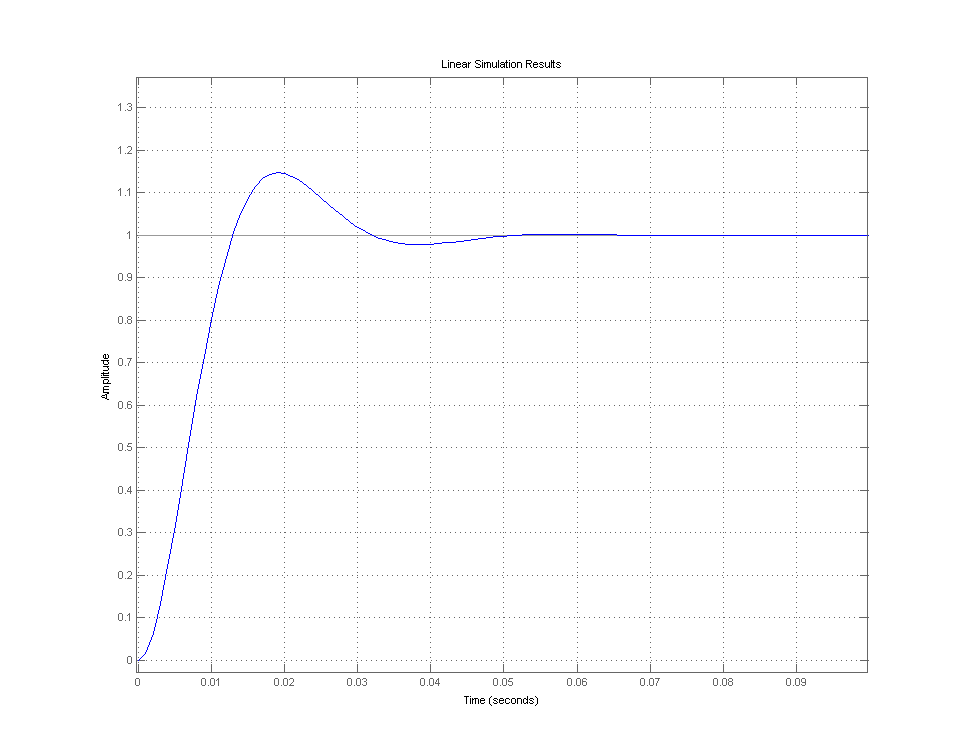
\includegraphics[scale=0.6,page=1]{6_зад/скачок_подобранная_2}

	В данном случае время регулирования $t_{\text{р}} = 0.028$ с, перерегулирование $\sigma_{\max} = 15 \%$.

	
	
\end{document}